% questions.tex —— 2008 年·春季上海卷 · 题目内容片段（无答案）
% 由 tools/generate_projects.py 依来源总账自 2008/2008_数学真题_春季上海_试题.md 生成，勿手改（改源 MD 后重跑）


\begin{gktip}
\textbf{来源说明}：按固定候选 PDF 第 1–2 页转录并目视核对；候选固定为本库当前工作输入，不认证出版者、版次、来源链或官方身份。PDF 共 4 页，第 3–4 页载有副本印载的参考答案与解答，但其归属和官方性未核实。答案与解析以独立推导为据，Q8 题面“凹多面体”与印载体积正负号冲突，答案保留 U，见独立盲解与对照及Q8 来源核查。

\textbf{页码映射}：PDF 第 1 页（印刷页 2-35）为填空题第 1–12 题及选择题第 13–15 题；第 2 页（印刷页 2-36）为选择题第 16 题与解答题第 17–22 题；后两页为副本印载答案，不属于本题面转录范围。图 1–3 按原件拓扑重绘为 TikZ 矢量示意。
\end{gktip}

\gkpart{卷首与题型说明（PDF 第 1 页，印刷页 2-35）}

2008 年上海市普通高等学校春季招生考试，数学试卷。试卷共 22 道试题，满分 150 分，考试时间 120 分钟。

\begin{itemize}
\item 一、填空题：12 题，共 48 分；每题填对得 4 分，否则得零分。
\item 二、选择题：4 题，共 16 分；每题四个结论中有且只有一个正确，选对得 4 分，否则得零分。
\item 三、解答题：6 题，共 86 分，须写出必要步骤。
\end{itemize}

\gkpart{一、填空题}

\begin{question}
\gkti{1}\textbf{（4 分）} 已知集合
\nopagebreak[4]
\[
A=\{x\mid x<-1\text{ 或 }2\le x<3\},\qquad B=\{x\mid -2\le x<4\},
\]
则 \(A\cup B=\underline{\qquad\qquad}\)。

\end{question}
\begin{question}
\gkti{2}\textbf{（4 分）} 计算
\nopagebreak[4]
\[
\lim_{n\to\infty}\frac{3^n+1}{3^{n+1}+2^n}=\underline{\qquad\qquad}\text{。}
\]

\end{question}
\begin{question}
\gkti{3}\textbf{（4 分）} 函数
\nopagebreak[4]
\[
f(x)=\frac{\sqrt{-x^2+x+6}}{x-1}
\]
的定义域是 \(\underline{\qquad\qquad}\)。

\end{question}
\begin{question}
\gkti{4}\textbf{（4 分）} 方程
\nopagebreak[4]
\[
2\cos\left(x-\frac\pi4\right)=1
\]
在区间 \((0,\pi)\) 内的解是 \(\underline{\qquad\qquad}\)。

\end{question}
\begin{question}
\gkti{5}\textbf{（4 分）} 已知数列 \(\{a_n\}\) 是公差不为零的等差数列，\(a_1=1\)。若 \(a_1\text{、}a_2\text{、}a_5\) 成等比数列，则 \(a_n=\underline{\qquad\qquad}\)。

\end{question}
\begin{question}
\gkti{6}\textbf{（4 分）} 化简
\nopagebreak[4]
\[
\cos\left(\frac\pi3+\alpha\right)+\sin\left(\frac\pi6+\alpha\right)=\underline{\qquad\qquad}\text{。}
\]

\end{question}
\begin{question}
\gkti{7}\textbf{（4 分）} 已知 \(P\) 是双曲线
\nopagebreak[4]
\[
\frac{x^2}{a^2}-\frac{y^2}{9}=1
\]
右支上的一点，双曲线的一条渐近线方程为 \(3x-y=0\)。设 \(F_1\text{、}F_2\) 分别为双曲线的左、右焦点。若 \(|PF_2|=3\)，则 \(|PF_1|=\underline{\qquad\qquad}\)。

\Needspace{0.4\textheight}
\end{question}
\begin{question}
\gkti{8}\textbf{（4 分）} 已知一个凹多面体共有 9 个面，所有棱长均为 1，其平面展开图如图 1 所示，则该凹多面体的体积 \(V=\underline{\qquad\qquad}\)。
\nopagebreak[4]
\begin{center}% Q8：固定副本中的展开图拓扑；所有小面边长均为 1。
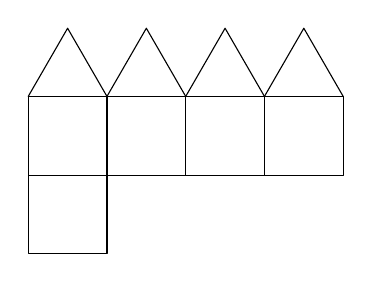
\begin{tikzpicture}[line cap=round,line join=round]
  % 四个侧方形依次相连，底方面连接在最左侧方形下边。
  \draw (0,0) rectangle (1,1);
  \draw (1,0) rectangle (2,1);
  \draw (2,0) rectangle (3,1);
  \draw (3,0) rectangle (4,1);
  \draw (0,-1) rectangle (1,0);
  % 四个等边三角形分别接在侧方形上边。
  \draw (0,1)--(0.5,1.866)--(1,1);
  \draw (1,1)--(1.5,1.866)--(2,1);
  \draw (2,1)--(2.5,1.866)--(3,1);
  \draw (3,1)--(3.5,1.866)--(4,1);
\end{tikzpicture}
\end{center}
\nopagebreak[4]
\end{question}
\begin{question}
\gkti{9}\textbf{（4 分）} 已知无穷数列 \(\{a_n\}\) 前 \(n\) 项和
\nopagebreak[4]
\[
S_n=\frac13a_n-1,
\]
则数列 \(\{a_n\}\) 的各项和为 \(\underline{\qquad\qquad}\)。

\end{question}
\begin{question}
\gkti{10}\textbf{（4 分）} 古代“五行”学说认为：“物质分金、木、水、火五种属性，金克木，木克土，土克水，水克火，火克金。”将五种不同属性的物质任意排成一列，设事件 \(A\) 表示“排列中属性相克的两种物质不相邻”，则事件 \(A\) 出现的概率是 \(\underline{\qquad\qquad}\)（结果用数值表示）。本题文字跨 PDF 第 1 页双栏。

\Needspace{0.4\textheight}
\end{question}
\begin{question}
\gkti{11}\textbf{（4 分）} 已知 \(a_1,a_2,\ldots,a_n\text{；}\ b_1,b_2,\ldots,b_n\)（\(n\) 是正整数），令
\nopagebreak[4]
\[
L_1=b_1+b_2+\cdots+b_n,\quad L_2=b_2+b_3+\cdots+b_n,\quad
L_3=b_3+\cdots+b_n,\quad\ldots,\quad L_n=b_n\text{。}
\]
\Needspace{5\baselineskip}
某人用图 2 分析得到恒等式
\nopagebreak[4]
\[
a_1b_1+a_2b_2+\cdots+a_nb_n
=a_1L_1+c_2L_2+c_3L_3+\cdots+c_kL_k+\cdots+c_nL_n\text{，}
\]
则 \(c_k=\underline{\qquad\qquad}\)（\(2\le k\le n\)）。
\nopagebreak[4]
\begin{center}% Q11：阶梯面积分块示意；后续项以省略号表示。
\begin{tikzpicture}[line cap=round,line join=round]
  \draw[->] (-0.15,0)--(5.85,0) node[right] {$x$};
  \draw[->] (0,-0.15)--(0,3.2) node[above] {$y$};
  \draw (0,0) rectangle (1,0.7);
  \draw (1,0) rectangle (2,1.2);
  \draw (2,0) rectangle (3,1.7);
  \draw (4,0) rectangle (5,2.5);
  \draw (1,0)--(1,-0.18);
  \draw (2,0)--(2,-0.18);
  \draw (3,0)--(3,-0.18);
  \draw (4,0)--(4,-0.18);
  \draw (5,0)--(5,-0.18);
  \node[below=4pt] at (0,0) {$O$};
  \node at (0.5,0.35) {$a_1$};
  \node at (1.5,0.6) {$a_2$};
  \node at (2.5,0.85) {$a_3$};
  \node at (3.5,1.25) {$\cdots$};
  \node at (4.5,1.25) {$a_n$};
  \node[below=15pt] at (0.5,0) {$b_1$};
  \node[below=15pt] at (1.5,0) {$b_2$};
  \node[below=15pt] at (2.5,0) {$b_3$};
  \node[below=15pt] at (3.5,0) {$\cdots$};
  \node[below=15pt] at (4.5,0) {$b_n$};
\end{tikzpicture}
\end{center}
\nopagebreak[4]
\end{question}
\begin{question}
\gkti{12}\textbf{（4 分）} 已知 \(A(1,2),\ B(3,4)\)，直线
\nopagebreak[4]
\[
l_1:x=0,\qquad l_2:y=0,\qquad l_3:x+3y-1=0\text{。}
\]
设 \(P_i\) 是 \(l_i\ (i=1,2,3)\) 上与 \(A\text{、}B\) 两点距离平方和最小的点，则 \(\triangle P_1P_2P_3\) 的面积是 \(\underline{\qquad\qquad}\)。

\end{question}
\gkpart{二、选择题}

本大题共 4 题，每题只有一个正确结论；正确结论的代号须写在题后的括号内。

\begin{question}
\gkti{13}\textbf{（4 分）} 已知向量 \(\vec a=(2,-3),\ \vec b=(3,\lambda)\)，若 \(\vec a\parallel\vec b\)，则 \(\lambda\) 等于\mbox{（　　）}。

\begin{itemize}
\item （A）\(\frac23\)　（B）\(-2\)　（C）\(-\frac92\)　（D）\(-\frac23\)
\end{itemize}

\end{question}
\begin{question}
\gkti{14}\textbf{（4 分）} 已知椭圆
\nopagebreak[4]
\[
\frac{x^2}{10-m}+\frac{y^2}{m-2}=1
\]
的长轴在 \(y\) 轴上。若焦距为 4，则 \(m\) 等于\mbox{（　　）}。

\begin{itemize}
\item （A）4　（B）5　（C）7　（D）8
\end{itemize}

\end{question}
\begin{question}
\gkti{15}\textbf{（4 分）} 已知函数 \(f(x)\text{、}g(x)\) 定义在 \(\mathbb R\) 上，\(h(x)=f(x)\cdot g(x)\)，则“\(f(x)\text{、}g(x)\) 均为奇函数”是“\(h(x)\) 为偶函数”的\mbox{（　　）}。

\begin{itemize}
\item （A）充分不必要条件
\item （B）必要不充分条件
\item （C）充要条件
\item （D）既不充分也不必要条件
\end{itemize}

\end{question}
\begin{question}
\gkti{16}\textbf{（4 分；PDF 第 2 页，印刷页 2-36）} 已知 \(z\in\mathbb C\)，且 \(|z-2-2i|=1\)，\(i\) 为虚数单位，则 \(|z+2-2i|\) 的最小值是\mbox{（　　）}。

\begin{itemize}
\item （A）2　（B）3　（C）4　（D）5
\end{itemize}

\end{question}
\gkpart{三、解答题}

\begin{question}
\gkti{17}\textbf{（12 分）} 已知
\nopagebreak[4]
\[
\cos\theta=-\frac{\sqrt2}{3},\qquad \theta\in\left(\frac\pi2,\pi\right)\text{，}
\]
\Needspace{5\baselineskip}
求
\nopagebreak[4]
\[
\frac2{\sin 2\theta}-\frac{\cos\theta}{\sin\theta}
\]
的值。

\end{question}
\begin{question}
\gkti{18}\textbf{（12 分）} 在平面直角坐标系 \(xOy\) 中，\(A\text{、}B\) 分别为直线 \(x+y=2\) 与 \(x\text{、}y\) 轴的交点，\(C\) 为 \(AB\) 的中点。若抛物线 \(y^2=2px\ (p>0)\) 过点 \(C\)，求焦点 \(F\) 到直线 \(AB\) 的距离。

\end{question}
\begin{question}
\gkti{19}\textbf{（14 分）} 已知函数
\nopagebreak[4]
\[
f(x)=\log_2(2^x+1)\text{。}
\]
(1) 求证：函数 \(f(x)\) 在 \((-\infty,+\infty)\) 内单调递增；
\Needspace{5\baselineskip}
(2) 记 \(f^{-1}(x)\) 为函数 \(f(x)\) 的反函数。若关于 \(x\) 的方程
\nopagebreak[4]
   \[
   f^{-1}(x)=m+f(x)
   \]
   在 \([1,2]\) 上有解，求 \(m\) 的取值范围。

\Needspace{0.4\textheight}
\end{question}
\begin{question}
\gkti{20}\textbf{（14 分）} 本题共 2 小题，第 1 小题 6 分，第 2 小题 8 分。某厂根据市场需求开发折叠式小凳（如图 3 所示）。凳面为三角形的尼龙布，凳脚为三根细钢管。考虑到钢管的受力和人的舒适度等因素，设计小凳应满足：①凳子高度为 30 cm；②三根细钢管相交处的节点 \(O\) 与凳面三角形 \(ABC\) 重心的连线垂直于凳面和地面。
\nopagebreak[4]
\begin{center}% Q20：折叠凳结构示意，投影和长度均不按比例。
\begin{tikzpicture}[line cap=round,line join=round]
  % 三角形凳面 ABC 的透视轮廓。
  \coordinate (A) at (0,2.4);
  \coordinate (B) at (1.45,1.65);
  \coordinate (C) at (3.2,2.45);
  \coordinate (O) at (1.65,0.9);
  \draw[thick] (A)--(B)--(C)--cycle;
  \node[above left] at (A) {$A$};
  \node[below] at (B) {$B$};
  \node[above right] at (C) {$C$};
  % 三根钢管由凳面顶点延至交点 O，并向地面方向伸出。
  \draw[thick] (A)--(O)--(2.8,-0.45);
  \draw[thick] (B)--(O)--(0.1,-0.5);
  \draw[thick] (C)--(O)--(2.05,-0.65);
  \fill (O) circle (1.5pt);
  \node[right] at (O) {$O$};
  \draw[dashed] (O)--(1.65,0.2);
  \draw (0,-0.55)--(3.1,-0.55);
  \node[right] at (3.1,-0.55) {地面};
\end{tikzpicture}
\end{center}
\nopagebreak[4]
(1) 若凳面是边长为 20 cm 的正三角形，三只凳脚与地面所成的角均为 \(45^\circ\)，确定节点 \(O\) 分细钢管上下两段的比值（精确到 0.01）；
(2) 若凳面是顶角为 \(120^\circ\) 的等腰三角形，腰长为 24 cm，节点 \(O\) 分细钢管上下两段之比为 \(2:3\)，确定三根细钢管的长度（精确到 0.1 cm）。

\end{question}
\begin{question}
\gkti{21}\textbf{（16 分）} 本题共 3 小题，第 1 小题满分 3 分，第 2 小题满分 5 分，第 3 小题满分 8 分。在直角坐标平面 \(xOy\) 上有一列点
\nopagebreak[4]
\[
A_1(1,a_1),\ A_2(2,a_2),\ \ldots,\ A_n(n,a_n),\ \ldots\text{，}
\]
\Needspace{5\baselineskip}
简记为 \(\{A_n\}\)。若
\nopagebreak[4]
\[
b_n=\overrightarrow{A_nA_{n+1}}\cdot\vec j
\]
构成的数列 \(\{b_n\}\) 满足 \(b_{n+1}>b_n,\ n=1,2,3,\ldots\)，其中 \(\vec j\) 是方向与 \(y\) 轴正方向相同的单位向量，则称 \(\{A_n\}\) 为 \(T\) 点列。

(1) 判断 \(A_1(1,1), A_2(2,\frac12), A_3(3,\frac13),\ldots,A_n(n,\frac1n),\ldots\) 是否为 \(T\) 点列，并说明理由；
(2) 若 \(\{A_n\}\) 为 \(T\) 点列，且点 \(A_2\) 在点 \(A_1\) 的右上方，任取其中连续三点 \(A_k\text{、}A_{k+1}\text{、}A_{k+2}\)，判断 \(\triangle A_kA_{k+1}A_{k+2}\) 的形状（锐角三角形、直角三角形、钝角三角形），并予以证明；
\Needspace{5\baselineskip}
(3) 若 \(\{A_n\}\) 为 \(T\) 点列，正整数 \(1\le m<n<p<q\) 满足 \(m+q=n+p\)，求证
\nopagebreak[4]
   \[
   \overrightarrow{A_nA_q}\cdot\vec j>\overrightarrow{A_mA_p}\cdot\vec j\text{。}
   \]

\end{question}
\begin{question}
\gkti{22}\textbf{（18 分）} 本题共 3 小题，分值依次为 4、6、8 分。已知 \(z\) 是实系数方程
\nopagebreak[4]
\[
x^2+2bx+c=0
\]
的虚根，记它在直角坐标平面上的对应点为 \(P_z(\operatorname{Re}z,\operatorname{Im}z)\)。

\Needspace{5\baselineskip}
(1) 若 \((b,c)\) 在直线 \(2x+y=0\) 上，求证：\(P_z\) 在圆
\nopagebreak[4]
   \[
   C_1:(x-1)^2+y^2=1
   \]
   上；
\Needspace{5\baselineskip}
(2) 给定圆
\nopagebreak[4]
   \[
   C:(x-m)^2+y^2=r^2\qquad(m\in\mathbb R,\ r\in\mathbb R,\ r>0)\text{，}
   \]
   则存在唯一的线段 \(s\) 满足：①若 \(P_z\) 在圆 \(C\) 上，则 \((b,c)\) 在线段 \(s\) 上；②若 \((b,c)\) 是线段 \(s\) 上一点（非端点），则 \(P_z\) 在圆 \(C\) 上。写出线段 \(s\) 的表达式，并说明理由；
(3) 由（2）知线段 \(s\) 与圆 \(C\) 之间确定了一种对应关系，通过这种对应关系的研究，填写表一（表中 \(s_1\) 是（1）中圆 \(C_1\) 的对应线段）。

\begin{center}
\begin{tabular}{ll}
\toprule
线段 \(s\) 与线段 \(s_1\) 的关系 & \(m\text{、}r\) 的取值或表达式 \\
\midrule
\(s\) 所在直线平行于 \(s_1\) 所在直线 &  \\
\(s\) 所在直线平分线段 \(s_1\) &  \\
线段 \(s\) 与线段 \(s_1\) 长度相等 &  \\
\bottomrule
\end{tabular}
\end{center}

\end{question}